\chapter{Introduction}
\label{introduction}

%\section{General Introduction}
%\section{Technologies Used}
%	\subsection{Why TensorFlow?}	
%	\subsection{Why Raspberry}		
%	\subsection{Why Pyhton?}
%\section{Objectives}				  **
%	\subsection{Primary Objectives}	  **
%	\subsection{Secondary Objectives} **
%\section{Motivation}


\section{General Introduction}
Humans have used body characteristics such as face, voice or even gait for thousands of years to recognize each other. Back in the 19th century Alphonse Bertillon (chief of the criminal identification division of the police department in Paris, France) laid the foundation of biometrics by his idea of using a number of body measurements to identify criminals. However, his idea lost popularity by the far more practical discovery of the distinctiveness of human fingerprints (\cite{jain_biometrics}).

Time has passed since that discovery, and technology has advanced enough to do the work of recognition by itself, no humans are needed. In this project we are going to use one kind of recognition that has been limited for a long time by technology and processing power of computers: face recognition. Fortunately in the last years the Google Brain team developed TensorFlow, an open source library for face recognition based in deep learning and written in Python, doing the task a bit easier. Using this library, this project sets out to build an \textit{intelligent assistant} that will recognise the user's face.

But this is not the only task of the assistant. As an Erasmus student I have seen how difficult could be to come to a new University. First days are caotic and you do not know anything about the campus, so even with the help from the University staff, finding the room of your next class can become an adventure. That is why this project will be aimed to help Erasmus students, identifying them by the face recognition and then showing them their timetable and the route to the room of their next class.

\section{Technologies Used}	

	\subsection{Why TensorFlow?}
	We have talked about TensorFlow as it would be the only library available, but there are many more, some of them even written also in Pyhton (e.g. \cite{theano_main_site}, \cite{caffe_main_site}). That said, why choose it instead other deep learning library? First, TensorFlow is one of the newest libraries at the moment of writing for deep learning in Python and we want this project to deal with a current issue. And second, this library has two APIs (\cite{tensorflow_main_website}): a high level API (MNIST), which makes it accessible for everyone and it will be easy to start with; and a low level API (Deep MNIST), which can provide a more advanced control for the final development of the project.

	\subsection{Why Raspberry Pi?}
	TensorFlow still needs a computer with a certain computing power, which also means that it will have a considerable size. In order to provide mobility to the assistant, a client-server architecture is going to be used. In the server side is where face recognition and high computing requirement tasks are actually going to be executed, while the client side will act as the interface of the system. 

	As the client side will not require much computing power, Raspberry Pi becomes an option. With the size of a credit card, Raspberry Pi is a low-cost and barebones computer capable to work as a traditional desktop tower. Many versions of this board have been released, but for this project we have chosen the Raspberry Pi 3 Model B.

	\begin{figure}[ht]
		\centering
		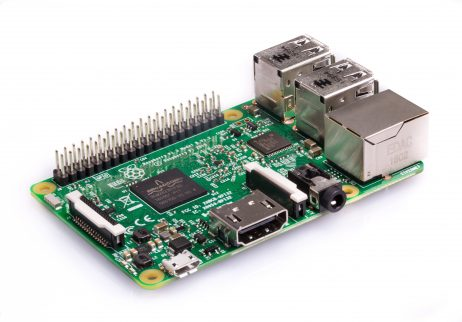
\includegraphics{raspberry-pi-3-b.jpg}
		\caption{Raspberry Pi 3, model B}
	\end{figure}

	Here we have its specifications:

	\subsection{Why Python?}
	The reasons that made Python the language chosen for this project were many. First, it is the language that Tensorflow uses to express the model of the network, so it was necessary to use it at least for the face recognition module of the project. Second, Python has become a widely used language because (\cite{why_python}):

	\begin{itemize}
		\item Proven language. Python is used by many important companies, such as Dropbox, Google or Amazon. 
		\item Fast prototypes. Python's dynamic nature and simple syntax make it perfect for prototyping, preventing us from worrying about the actual implementation and helping to focus on data and algorithms, which the main task of machine learning.
		\item For everyone. Many data scientist and engineers have a background in maths and statistics, but they may not have any experience in programming. Python's simplicity and readability, as it is said to have a math-like syntax, make it easier to pick up.
		\item Mature Data Science Ecosystem. There is a great collection of math and data science for Python, incremented by new libraries that are built on top of the older ones (but controlled by the solid Python's packaging). 
	\end{itemize}

	Finally, the last reason is personal. During the last years in my home University, I heard many times how important Python was and how popular it was becoming. However, the modules from my study program never used this language for their assignments, so I never had the opportunity to learn it in an academic environment. Because of that, I decided to use Python in all aspects of this project in order to learn how to work with it.  

\section{Objectives}
	\subsection{Primary Objectives}
	\subsection{Secondary Objectives}

\section{Motivation}
The use of face recognition have experimented an incredible rise in the last times. Not long ago we saw how Apple brought out the new iPhoneX. This new model says goodbye to the usual ways to unblock the terminal (e.g. codes, patterns or fingerprints) incorporating the FaceID software, which is nothing but a face recognition approach. This may be a more known case of face recognition, but as we see in \cite{iphonex_and_other_uses}, it is already used around the world to examine, investigate, and monitor. For example in China, police use it to identify the people who commit the crime of jaywalking. In the United States, more than a half of all American adults are in a face recognition database that can be used for criminal investigations (thanks to their driver’s license).





